% !TEX TS-program = xelatex
% !TEX encoding = UTF-8 Unicode

\documentclass[AutoFakeBold]{LZUThesis}
\usepackage{wasysym}
\usepackage{enumitem}
\usepackage[most]{tcolorbox}
\usepackage{multirow}
\usepackage{tikz}
\usetikzlibrary{arrows.meta, decorations.markings}
\usepackage{hyperref}
\usepackage[numbers,sort&compress]{natbib}
\newcommand{\upcite}[1]{\textsuperscript{\textsuperscript{\cite{#1}}}}
\allowdisplaybreaks[4]

\begin{document}

\title{{实验二数据运算:定点乘法}}

\entitle{Experiment 2 Data Operation: Fixed-point Multiplication}

\author{生物信息学班 李泽华 320210928501}
\major{计算机组成原理}
\advisor{高平}
\college{生命科学学院}
\grade{2021级}


\frontmatter

% \ZhAbstract{
% }{
% }

%\EnAbstract{
%}{
%}

\customcontent

\mainmatter

% \chapter{\texorpdfstring{绪 \quad 论}{绪论}}
\chapter{实验目的}
\begin{enumerate}
    \item 理解定点乘法的不同实现算法的原理,掌握基本实现算法。
    \item 熟悉并运用 verilog 语言进行电路设计。
    \item 为后续设计 cpu 的实验打下基础。
\end{enumerate}

\chapter{实验任务与要求}
\section{实验任务}
\begin{enumerate}
    \item 学习并理解计算机中定点乘法器的多种实现算法的原理,重点掌握迭代乘法的实现算法。
    \item 自行设计本次实验的方案,画出结构框图,详细标出输入输出端口,本次实验的乘法器建议采用迭代的方式实现,如果能力有余的,也可以采用其他效率更高的算法实现。本次实验要求实现的乘法为有符号乘法,因此需要注意计算机存储的有符号数都是补码的形式,设计方案传递进来的数也需是补码。
    \item 根据设计的实验方案,使用 verilog 编写相应代码。
    \item 对编写的代码进行仿真,得到正确的波形图。
    \item 将以上设计作为一个单独的模块,设计一个外围模块去调用该模块。外围模块中需调用封装好的 LCD 触摸屏模块,显示两个乘数和乘法结果,且需要利用触摸功能输入两个乘数。
    \item 将编写的代码进行综合布局布线,并下载到实验箱中的 FPGA 板子上进行演示。
\end{enumerate}
\section{实验要求}
\begin{enumerate}
    \item 做好预习:
    1) 掌握定点乘法的多种实现算法的原理;
    2) 确定定点乘法的输入输出端口设计;
    3) 在课前画好设计框图或实验原理图;
    4) 如果对 FPGA 板了解的话,可确定设计中与 FPGA 板上交互的接口,画出包含外围模块的整体设计框图,即补充完善图 3.1。
    \item 实验实施:
    1) 确认定点乘法的设计框图的正确性;
    2) 编写 verilog 代码;
    3) 对该模块进行仿真,得出正确的波形,截图作为实验报告结果一项的材料;
    4) 完成调用定点乘法模块的外围模块的设计,并编写代码;
    5) 对代码进行综合布局布线下载到实验箱里 FPGA 板上,进行上板验证。
    \item 实验检查:
    1) 完成上板验证后,让指导老师或助教进行检查,进行现场演示,可对演示结果进行拍照作为实验报告结果一项的材料。
    \item 实验报告的撰写:
    1) 实验结束后,需按照规定的格式完成实验报告的撰写。
\end{enumerate}

\chapter{实验结果}
最终代码:
\begin{lstlisting}[language=Verilog]
`timescale 1ns / 1ps
module multiply(              // 乘法器
    input         clk,        // 时钟
    input         mult_begin, // 乘法开始信号
    input  [31:0] mult_op1,   // 乘法源操作数1
    input  [31:0] mult_op2,   // 乘法源操作数2
    output [63:0] product,    // 乘积
    output        overflow,   // 溢出
    output        mult_end    // 乘法结束信号
);

    //乘法正在运算信号和结束信号
    reg mult_valid;
    assign mult_end = mult_valid & ~(|multiplier); //乘法结束信号:乘数全0
    always @(posedge clk)
    begin
        if (!mult_begin || mult_end) //乘法未开始或者乘法结束
        begin
            mult_valid <= 1'b0; //乘法无效
        end
        else
        begin
            mult_valid <= 1'b1; //乘法有效
        end
    end

    //两个源操作取绝对值,正数的绝对值为其本身,负数的绝对值为取反加1
    wire        op1_sign;      //操作数1的符号位
    wire        op2_sign;      //操作数2的符号位
    wire [31:0] op1_absolute;  //操作数1的绝对值
    wire [31:0] op2_absolute;  //操作数2的绝对值
    assign op1_sign = mult_op1[31];
    assign op2_sign = mult_op2[31];
    assign op1_absolute = op1_sign ? (~mult_op1+1) : mult_op1;
    assign op2_absolute = op2_sign ? (~mult_op2+1) : mult_op2;

    //加载被乘数,运算时每次左移一位
    reg  [63:0] multiplicand;
    always @ (posedge clk)
    begin
        if (mult_valid)
        begin    // 如果正在进行乘法,则被乘数每时钟左移一位
            multiplicand <= {multiplicand[62:0],1'b0};
        end
        else if (mult_begin) 
        begin   // 乘法开始,加载被乘数,为乘数1的绝对值
            multiplicand <= {32'd0,op1_absolute};
        end
    end

    //加载乘数,运算时每次右移一位
    reg  [31:0] multiplier;
    always @ (posedge clk)
    begin
        if (mult_valid)
        begin   // 如果正在进行乘法,则乘数每时钟右移一位
            multiplier <= {1'b0,multiplier[31:1]}; 
        end
        else if (mult_begin)
        begin   // 乘法开始,加载乘数,为乘数2的绝对值
            multiplier <= op2_absolute; 
        end
    end
    
    // 部分积:乘数末位为1,由被乘数左移得到;乘数末位为0,部分积为0
    wire [63:0] partial_product;
    assign partial_product = multiplier[0] ? multiplicand : 64'd0;
    
    //累加器
    reg [63:0] product_temp;
    always @ (posedge clk)
    begin
        if (mult_valid)
        begin
            product_temp <= product_temp + partial_product;
        end
        else if (mult_begin) 
        begin
            product_temp <= 64'd0;  // 乘法开始,乘积清零 
        end
    end 
     
    //乘法结果的符号位和乘法结果
    reg product_sign;
    always @ (posedge clk)  // 乘积
    begin
        if (mult_valid)
        begin
            product_sign <= op1_sign ^ op2_sign;
        end
    end 
    

    // 若乘法结果为负数,则需要对结果取反+1
    assign product = product_sign ? (~product_temp+1) : product_temp;

    // 检测溢出
    // 当乘法结果大于2^31-1或小于-2^31时,溢出
    assign overflow = product > 64'h7fffffff || product < -64'h80000000;

    endmodule

\end{lstlisting}

\chapter{思考与讨论}
\section{课后问题}
\begin{enumerate}
    \item 以4位二进制数1010和0110为源操作数1和源操作数2,手工完成计算过程
    \[
    \begin{array}{ c c c c c c c c }
        & & & & 1 & 0 & 1 & 0 \\
        \times & & & & 0 & 1 & 1 & 0 \\
        \hline
        & & & & 0 & 0 & 0 & 0 \\
        & & & 1 & 0 & 1 & 0 & \\
        & & 1 & 0 & 1 & 0 &  &  \\
        + & 0 & 0 & 0 & 0 & & & \\
        \hline
        & 0 & 1 & 1 & 1 & 1 & 0 & 0
    \end{array}
    \]
    \item 判断乘法器的有效输入为有符号数还是无符号数?尝试更改为另一种有效输入方案 \\
    乘法器的有效输入为有符号数,因为乘法器的输入是有符号数,输出也是有符号数 \\
    更改为无符号数: \\
    \begin{lstlisting}[language=Verilog]
module multiply(
    input         clk,
    input         mult_begin,
    input  [31:0] mult_op1,   // 改为无符号数
    input  [31:0] mult_op2,   // 改为无符号数
    output [63:0] product,
    output        mult_end
);

    // 乘法正在运算信号和结束信号
    reg mult_valid;
    assign mult_end = mult_valid & ~(|multiplier);
    always @(posedge clk) begin
        if (!mult_begin || mult_end)
            mult_valid <= 1'b0;
        else
            mult_valid <= 1'b1;
    end

    // 加载被乘数,运算时每次左移一位
    reg  [63:0] multiplicand;
    always @ (posedge clk) begin
        if (mult_valid)
            multiplicand <= {multiplicand[62:0], 1'b0};
        else if (mult_begin)
            multiplicand <= {32'd0, mult_op1}; // 无需绝对值处理
    end

    // 加载乘数,运算时每次右移一位
    reg  [31:0] multiplier;
    always @ (posedge clk) begin
        if (mult_valid)
            multiplier <= {1'b0, multiplier[31:1]}; 
        else if (mult_begin)
            multiplier <= mult_op2; // 无需绝对值处理
    end
    
    // 部分积
    wire [63:0] partial_product;
    assign partial_product = multiplier[0] ? multiplicand : 64'd0;
    
    // 累加器
    reg [63:0] product_temp;
    always @ (posedge clk) begin
        if (mult_valid)
            product_temp <= product_temp + partial_product;
        else if (mult_begin)
            product_temp <= 64'd0;
    end 
    
    // 乘法结果
    assign product = product_temp;

endmodule
    \end{lstlisting}        

    \item 对仿真结果(波形图)进行注释
    \begin{figure}[htbp]
        \centering
        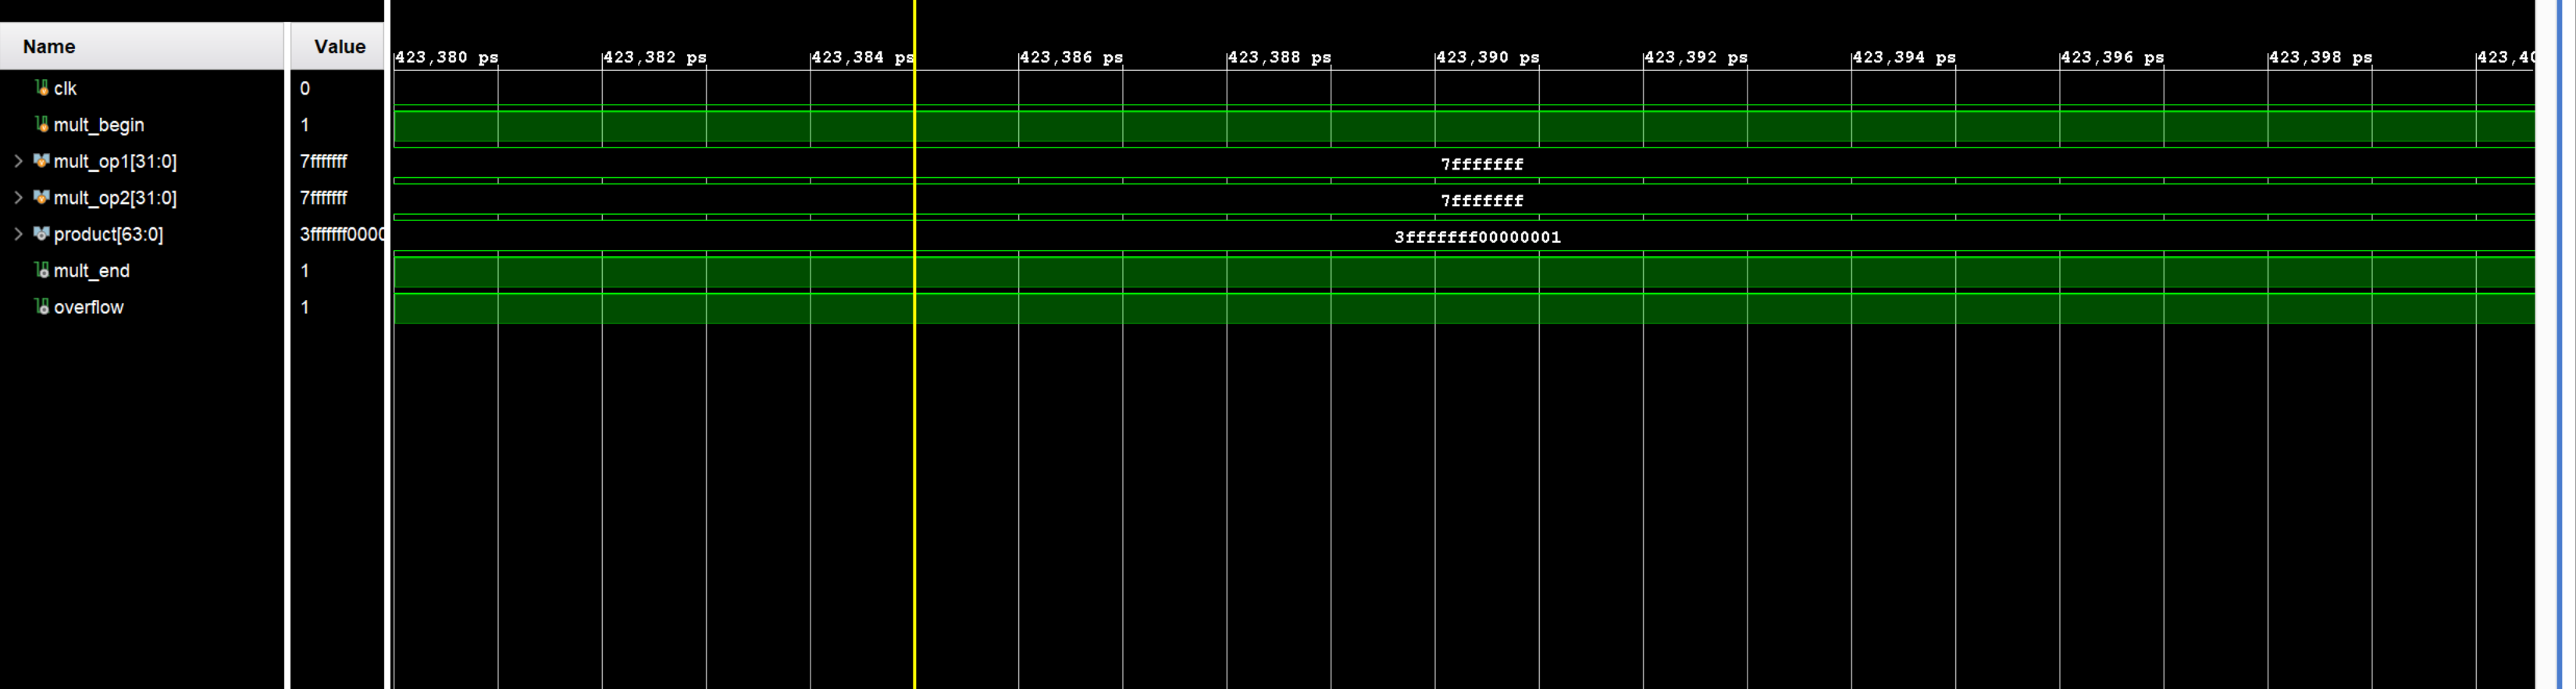
\includegraphics[width=0.8\textwidth]{img/img}
        \caption{乘法器波形图}
    \end{figure}
    \begin{enumerate}
        \item mult\_begin信号在第一个时钟上升沿变为1,表示乘法开始
        \item mult\_end信号在第四个时钟上升沿变为1,表示乘法结束
        \item mult\_op1和mult\_op2在第一个时钟上升沿变为7fffffff, 7fffffff
        \item product在第四个时钟上升沿变为3fffffff00000001
        \item overflow为1,表示溢出
    \end{enumerate}
    \item 说明mult\_begin信号最终由什么(实验箱)确定

    根据代码中的逻辑,当 mult\_begin 为高电平时,表示乘法操作应该开始。而 mult\_begin 信号的状态受到外部时钟信号 clk 的影响,并且还受到其他输入信号 mult\_op1 和 mult\_op2 的状态的影响。只有当 mult\_begin 为高电平且其他条件满足时,乘法操作才会开始。
    \item 给出乘法器溢出标志位(按有符号数计算处理),提交代码
    \begin{lstlisting}[language=Verilog]
    module multiply(          // 乘法器
    input         clk,        // 时钟
    input         mult_begin, // 乘法开始信号
    input  [31:0] mult_op1,   // 乘法源操作数1
    input  [31:0] mult_op2,   // 乘法源操作数2
    output [63:0] product,    // 乘积
    output        overflow,   // 溢出
    output        mult_end    // 乘法结束信号
);

    //......

    // 当乘法结果大于2^31-1或小于-2^31时,溢出
    assign overflow = product > 64'h7fffffff || product < -64'h80000000;
    \end{lstlisting}
\end{enumerate}
%论文后部
\backmatter


%=======%
%引入参考文献文件
%=======%
%\bibdatabase{bib/database}%bib文件名称 仅修改bib/ 后部分
%\printbib
%\nocite{*} %显示数据库中有的,但是正文没有引用的文献



\Appendix
参考链接:
\url{https://github.com/zehua0417/ComputerOrganizationAndArchitecture_exp}

%\Thanks


%\Grade %这一句才是成绩页,上面是填写


\end{document}
